\chapter{Introduction}
With the maturity of database technologies, nowadays
applications collect data in all domains at an
unprecedented scale. For example, billions of 
social network users and their activities are collected in the form
of \emph{graphs}; Thousand sensor reports are collected per second
in the form of \emph{time series}; Hundreds of millions of temporal-locations
are collected as \emph{trajectories}, to name just a few. Flooded by the
tremendous amount of data, it is emerging to 
provide useful and efficient analytics for various data domains.
Traditional SQL-based analytics which comprises 
of primitives (such as, partition, sorting and aggregation etc.)
become limited in non-structured data domains.
In SQL context, interesting analytics such as graph traversal and pattern detection
often involve complex joins which are very hard to optimize 
without domain knowledge.
In this thesis, we explore the neighborhood data analytic, which
in SQL is expressed by the window function,
on different data domains and demonstrate how to efficiently deploy
neighborhood data analytic to gain useful data insights.
%
%Traditional SQL-based analytics including ranking, aggregation, 
%and window functions, has seen a great success in supporting
%data-based decision-makings on relational data. However, 
%when applying SQL-based analytics on other data domains, it often
%involves expensive joins which are hard to optimize without leveraging the domain
%knowledge. For instance, when computing the $K$-hop neighborhoods of vertexes in a graph, 
%SQL-based traversal of graph involves multi-rounds of joins, which is inefficient
%than search-based traversal~\cite{}. Or, when searching for a group of objects
%that travels together for a certain time, SQL-based solution would involves
%recursive joins and chain joins.
%
%See from the limitation of SQL-analytic on those domains, in this thesis, we 
%explore the neighborhood based analytics in various data domains.
%In particular, we address three issues. First, we define the neighborhoods
%on various domains. Second, we showcase the usefulness of neighborhood analytics 
%on data models.
%Third, we address the efficiency issues on applying the neighborhood
%analytics in different data domains for large data.

% 
%With the rapid advancement of technologies, 
%many applications nowadays generate floods of data. 
%For example, social network users and their
%activities generate graph data; News events generate
%streams of texts; and moving vehicles generate spatial-temporal trajectories.
%These data embeds a wealth of information from different domains 
%which is crucial in supporting data-driven decision-makings. An 
%important tasks in management of these data is to provide useful analytics
%to facilitate the discovery of data insights. Thus, the design of 
%effective methods for data analysis under different application domains 
%has drawn a tremendous attention from both industries and academia recently.
%
%Traditional SQL-defined analytics which are specifically designed for
%structured data faces two major issues in supporting data analytics under
%various domains. First, SQL analytics has limited operations which may not
%be suitable for some applications. Second, SQL analytics may loose semantic
%meaning in no-structured or semi-structured data.

%Traditionally,  SQL-defined analytics becomes limited when handling data with such heterogeneity.
%Opposed to the one-set-fits-all SQL analytics,
%ad-hoc analytics for each domain are often required.
% Thus, the design
%of 
%
%An important aspect in data analytics is to study the data objects
%that are locally connected, as these data demonstrates strong clustering features. Such a kind 
%of analytic is referred as \emph{neighborhood analytic}. Nevertheless, the neighborhood
%analytic is prevalently seen in many area of applications.


 
%
%nowadays data are collected 
%at unprecedented scale. With the heterogeneity of data, many
%decisions that are painstakingly constructed manually 
%increasingly rely on data insights. 
%A crucial taks in management of such data is to provide useful analytics to 
%With the whole suite of the SQL analytic tools, data-driven decisions are 
%
%Decisions that previously were based on guesswork, or on	
%painstakingly constructed models of reality, can now be made based on the data itself. 
%A crucial task in management of data is to provide useful
%analytics to facilitate the discovery of data insights.
%
%As we
%enter the era of ``Big-data'', traditional SQL 
%analytics, which are designed specifically for structural relational data,
%are becoming shorthanded in supporting data with heterogeneity. 
%
%We are awash in	a flood of data today.	 In	 a broad range of application areas, data is being	
%collected at unprecedented scale.	 	 Decisions that previously were based	 on guesswork, or	 on	
%painstakingly constructed models of reality, can now be made based on the data itself.	 Such Big Data	
%analysis now drives nearly every aspect of our	 modern society, including mobile services, retail,	
%manufacturing, financial	services, life sciences, and	physical	sciences.
%
%``Big-data'', famous for its heterogeneity, scale and complexity, 
%has entering to the research horizon with promising potential 
%in data-driven decision-making. There has been an increasing needs
%for analyzing, understanding and processing ``big-data'' from
%both industrial and academic perspective. 
%
%``Neighborhood'' based analytic has been a complementary method
%for analyze data from a local perspective, which plays an important
%role in traditional data analytics. For instance, density-based spatial
%clustering examines the ....  egocentric network analysis,  SQL window
%function... Semi-Lazy data mining,
%to name a few. While these analytics are successful in 
%traditional area, it is left unknown whether ``neighborhood'' 
%based analytic is able to discover more insights in Big-data era.
%
%
%As being part of the research efforts
%in closing the gap between the potential of ``big-data'' and its realization,
%this thesis investigates the possibility of introducing ``neighborhood''-based
%analytic to ``big-data'' analysis. Specifically, we propose and analyze
% ``neighborhood''-based analytic in three heterogeneous domains: graph data,
% stream data, and spatial-temporal data. We design ad-hoc ``neighborhood''
% based data analytic on each data domain, and demonstrate the effectiveness
% of these analytic. We further address the challenges of applying these
% analytic efficiently by designing efficient index, powerful pruning, and scalable systems.
%
%
%The promise	of data-driven decision-making is now being recognized broadly, 
%and there is growing enthusiasm for	the notion of ``Big Data''.	 
%While the promise of Big Data is real -- for example, it is 
%estimated that Google alone contributed	54 billion dollars to the US economy
%in 2009 -- there is	currently a wide gap between its potential and its realization.
%Heterogeneity, scale, timeliness, complexity, and	privacy	 problems
%with Big Data impede progress at all phases of the pipeline that can create value from data.
%The problems start right away during data acquisition, when the data tsunami requires us to make decisions, currently in an ad hoc	manner, about what data to keep and what to discard, and how to store what	we keep reliably	with the	
%right metadata.	 Much data today is not natively in structured format; for example, tweets	and blogs are	
%weakly structured pieces of text,	while images and video are structured for storage and display, but not	
%for semantic content and search: transforming such content into a structured format for later analysis is	
%a major challenge. The value of data explodes when it can be linked with other data, thus data	
%integration	is a	major	creator	of	value.	 Since most data is directly generated in	digital format today, we	
%have the opportunity and	 the challenge both	 to influence the creation	to facilitate later linkage and	 to	
%automatically link previously created	data.	 Data	analysis, organization, retrieval, and	modeling	are other	
%foundational challenges.	 Data analysis is a clear bottleneck in many applications, both due to lack of	
%scalability of the underlying algorithms and due to the complexity of the data	that needs to be analyzed.	
%Finally, presentation	of the results and its interpretation by non-technical domain experts is crucial to	
%extracting	actionable knowledge.

\section{Neighborhood Data Analytic}
By its self-describing name, neighborhood data analytic aims to provide
summaries of each object over its vicinity. In contrast to the global
analytics which aggregates the entire collection of data as a whole, neighborhood
data analytic provides a personalized view on each object per se. Neighborhood
data analytics originates from the window function defined in  SQL which is
illustrated in Figure~\ref{fig:window}.

\begin{figure}[h]
\centering
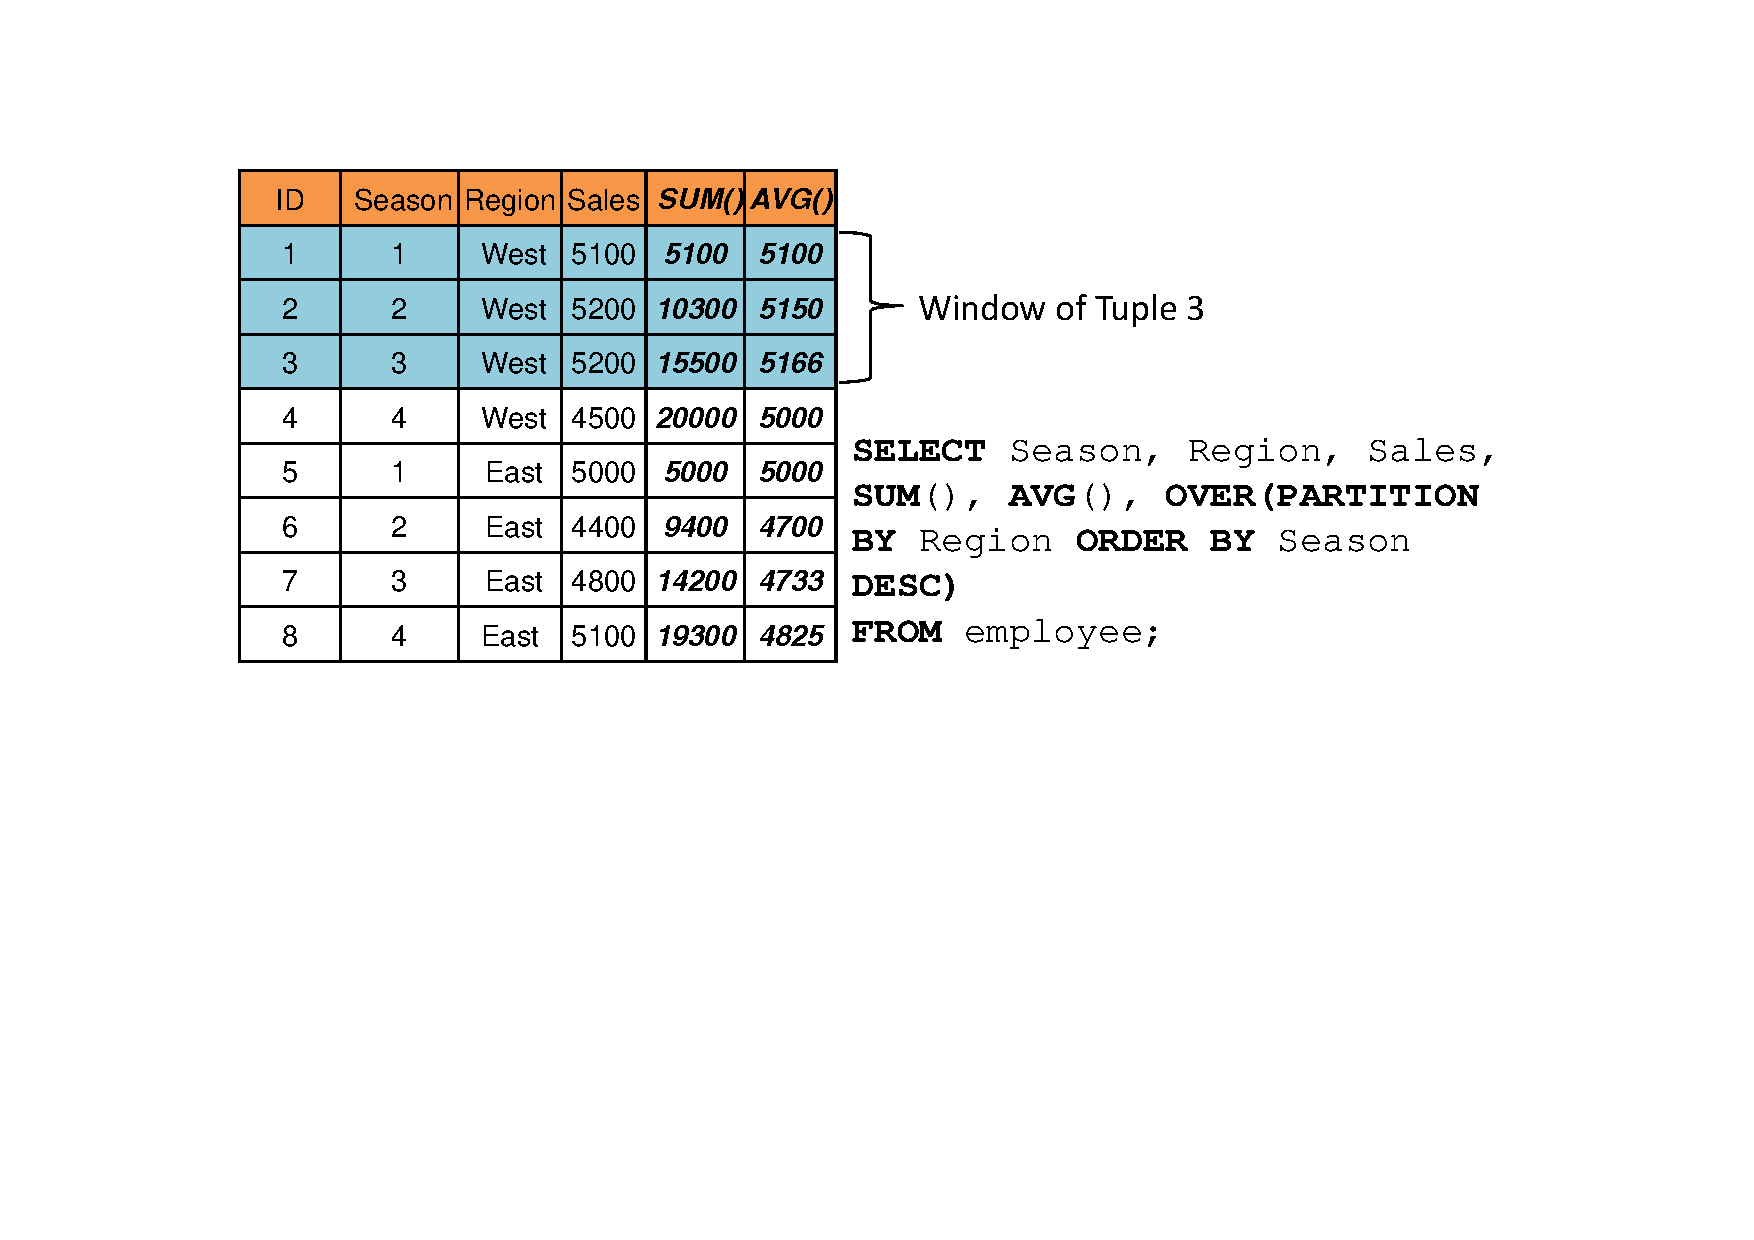
\includegraphics[width=0.8\linewidth]{window_example.pdf}
\caption{A SQL window function computing running sum and average of
sales. The window of season-3 is highlighted.} 
\label{fig:window}
\end{figure}

As shown in the figure,the sales report of a company contains five attributes. 
``Season'', ``Region'' and ``Sales'' are the original fields, ``$\mathtt{sum()}$'' and ``$\mathtt{avg()}$''
are the analytics representing the running sum and average. A window function
is represented by the $\mathtt{over}$ keyword. In this context, the window of a tuple $o_i$
contains other tuples $o_j$ such that $o_i$ and $o_j$ are in the same ``region'' and $o_j$'s ``season'' is
prior to $o_i$'s. The window of season-$3$ for region-``West'' is highlighted.

Apart from this example, there are many other 
usages of the window function in the relational context. 
Being aware of the success of the window function, 
SQL~11 standard incorporates ``$\mathtt{LEAD}$'' and ``$\mathtt{LAG}$'' 
keywords which offer fine-grained specifications on a tuple's window.

Despite the usefulness, there are few works reporting the window
analytics in the non-relational context. This may dues to the
usage of \emph{sorting} in relational windows. For example,
in Figure~\ref{fig:window},
objects needs to be sorted according to ``Season'', and then the windows of
each object are implicitly formed. However, 
in non-relational context, sorting may be ambiguous and undefined.

To generalize the window function to other data domains, we define the neighborhood
analytics in a broader context. Given a set of objects 
(such as tuples in relational context or vertexes in graph context),
the neighborhood analytic is a composite function
$(\mathcal{F} \circ \mathcal{N})$ applied on every object. $\mathcal{N}$
is the \emph{neighborhood function}, which contains the related objects of $o$;
$\mathcal{F}$ is an \emph{analytic function}, which could be aggregate, rank,
pattern matching, etc.
%the neighborhood analytic instance consists of two parts: a neighborhood indicator
%function $\mathbb{N}(o_i,o_j)$ deciding whether $o_j$ is in $o_i$'s neighborhoods,
%and an analytic function $f$ which aggregates a set of objects.  
%Let $N(o_i)$ be
%the set of neighbors of $o_i$, the neighborhood analytic aims to compute $f(N(o_i))$
%for all objects.
Apparently, relational window functions is a special case of such defined 
neighborhood analytics. For example, window function in Figure~\ref{fig:window} 
can be represented as $\mathcal{N}(o_i)=\{o_j | o_i.season > o_j.season \wedge o_i.region = o_j.region\}$
and $\mathcal{F} = \mathtt{avg}$.
Since the \emph{sorting} requirement is relaxed, our definition of neighborhood analytics
enriches the semantic of relational window notations 
and can be applied on other domains.
%
%Intuitively, we enrich the semantic of neighborhood as compared to the relation
%window notations. And our definition directly supports relational window notations by setting $\mathcal{N}$
%to capture the $\mathtt{over}$ clause. Since the \emph{sorting} is not required, such a 
%
%
%and is able to be
%applied on other data domains.


\section{Scope of the thesis}
In this thesis, we explore the neighborhood analytics in
different data domains. Our efforts showcase the usefulness of the neighborhood
concepts in those data domains and address the efficiency issues when adopting
nontrivial analytics. In particular, we looked at three most prevalent data domains, namely \textbf{graph},
\textbf{time series} and \textbf{trajectory}. 
We then categorize two intuitive neighborhood function $\mathcal{N}$ as follows:

\textbf{Distance Neighborhood}: the neighborhood is defined based on numeric distance, that is $\mathcal{N}(o) = \{o_i | \mathtt{dist}(o,o_i) \leq K \}$, where $\mathtt{dist}$ is a distance function and $K$ is a distance threshold.

\textbf{Comparison Neighborhood}: the neighborhood is defined based on the comparison of objects, that is $\mathcal{N}(o) = \{o_i | o.a_m \ \mathtt{op} \ o_i.a_m\}$, where $a_m$ is an attribute of object
and $\mathtt{op}$ is a binary comparator.

Due to the space limitation, we only consider the neighborhoods that is \emph{distance} or \emph{comparison} or any combinations of these two. In terms of analytic function $\mathcal{F}$, we consider aggregate, rank, and pattern matching.

\section{Contributions}
The high level contributions of this thesis are bi-folded. First, by
sewing different $\mathcal{N}$ and $\mathcal{F}$, three interesting
neighborhood analytic queries are proposed for \emph{graph}, \emph{trajectory}
and \emph{time series} data domains respectively. Second, this thesis
deals with the efficiency issues in deploying corresponding analytic queries to
handle data with nowadays scale.
The overview of this thesis is as show in Figure~\ref{fig:thesis_roadmap}.
\begin{figure}[h]
\centering
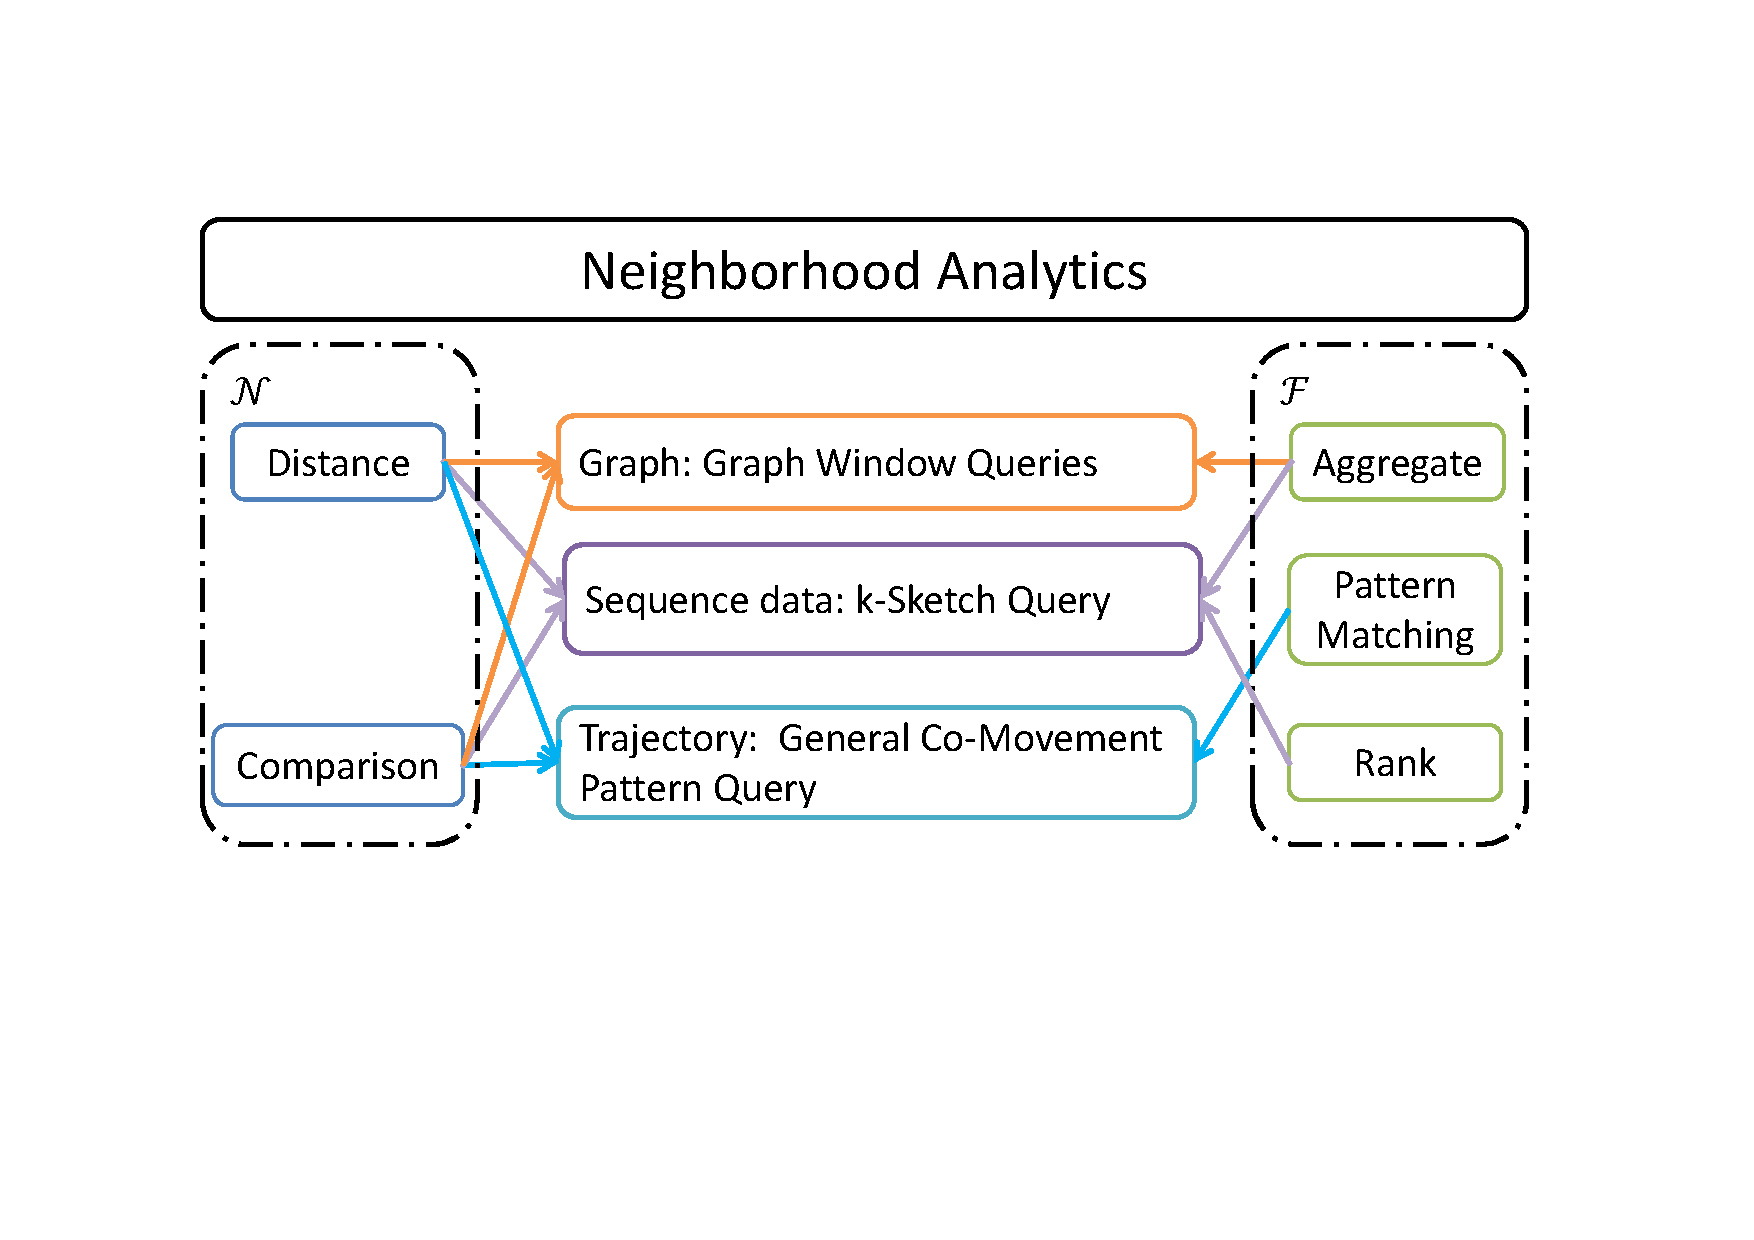
\includegraphics[width=0.8\linewidth]{thesis_roadmap.pdf}
\caption{The road map of this thesis. There are three major contributions as highlighted in the center. Each contribution
is a neighborhood analytic based on different $\mathcal{N}$ and $\mathcal{F}$ as indicated by arrows.} 
\label{fig:thesis_roadmap}
\end{figure}

\subsection{Graph Window Analytics}
This first piece of the thesis is on proposing neighborhood analytics
for graph data. Information networks such as social networks, biological networks
and phone-call networks are typically modeled as graphs where the 
vertexes correspond to objects and the edges capture the
relationships between these objects. 
In the context of graph, we 
the \emph{graph window analytics}. The window is essentially 
a neighborhood function. We have identified 
two instances of graph windows, namely
\emph{k-hop} and \emph{topological} windows. 
The \emph{k-hop} window is a \emph{distance} neighborhood function, i.e., $\mathcal{N}_k(v)= \{u|\mathtt{dist}(v,u) \leq K\}$, which captures the vertexes that are $k$-hop nearby. 
The \emph{topological} window,  $\mathcal{N}_t(v)= \{u | u \in v.ancestor\}$,
is a \emph{comparison} neighborhood function that captures
the ancestors of a vertex in a directly acyclic graph. 

With the two defined neighborhood function, we present many useful analytics. To support efficient graph window query processing, we propose
two different types of indexes: Dense Block Index (DBIndex)
and Inheritance Index (I-Index). The DBIndex and I-Index
are specially optimized to support k-hop window and topological
window query processing. We develop the indexes
by integrating the window aggregation sharing techniques
to salvage partial work done for efficient computation. 
In addition, we develop space and performance efficient techniques
for index construction. In our experiments, DBIndex saves upto 80\%
of indexing time as compared to the state-of-the-art competitor.


\subsection{Automatic News Discovery in Time Series Data}
The second piece of the thesis proposes a neighborhood analytic
query to automatic discover news in the time series data.
Automatic discovery of newsworthy themes from sequenced
data can relieve journalists from manually poring over a
large amount of data in order to discover interesting news.
An typical news themes generated from time-series data
is the so-called \emph{prominent streaks}. We resolve the limitations
of \emph{prominent streaks}.

Previous efforts have focused on generating prominent streaks
that are limited to single subjects. In this paper, we consider 
the prominence of a subject's streak in comparison to
the peers' and propose a novel scoring function that takes
into account both strikingness and diversity. Our objective
is to maintain the k most striking and representative news
themes for each subject. We study the problem in both
offline and online scenarios, and propose various window-
level pruning techniques to and striking candidate themes.
Among those candidates, we then develop approximation
methods, with theoretical bounds, to discover the k most
representative themes. We conduct experiments on four real
datasets, and the results demonstrate the efficiency and 
effectiveness of our proposed algorithms: the running time
achieves up to 500 times speedup and the quality of the
detected news themes is endorsed by the anonymous users
from Amazon Mechanical Turk.

\subsection{Mining Co-Movement in Trajectory Databases}
The third piece of the thesis is on trajectory.
Discovering co-movement patterns from large-scale trajectory 
databases is an important mining task and has a wide
spectrum of applications. Previous studies have identified
several types of interesting co-movement patterns and showcased 
their usefulness. In this paper, we make two key 
contributions to this research field. First, we propose a more
general co-movement pattern to unify those defined in the
past literature. Second, we propose two types of parallel and
scalable frameworks and deploy them on Apache Spark. To
the best of our knowledge, this is the first work to mine
co-movement patterns in real life trajectory databases with
hundreds of millions of points. Experiments on three real
life large-scale trajectory datasets have verified the efficiency
and scalability of our proposed solutions.

\section{Thesis Organization}
%The remaining part of the thesis are organized as follows: in Chapter 2, we summarize related literature. In Chapter 3, we present the window function of graph data using \emph{distance} and \emph{comparative} neighborhoods. In Chapter 4, we present a news discovery application on time series data using \emph{hybrid} neighborhoods. In Chapter 5, we present a pattern mining framework utilizing \emph{comparative} neighborhoods in trajectory data.